\chapter{Introduction}
\label{introduction}
 % start numberings at 0 because (computer) science
\setcounter{figure}{-1}
\setcounter{table}{-1}
\setcounter{section}{-1}
\setcounter{NAT@ctr}{-1}

\setlength\parindent{0pt}


\begin{comment}
\section*{Contents}
\begin{enumerate}
\itemsep-0.5em
\item A Brief History of Genomics
\item A Primer on Sequencing (?)
\item The Bioinformatics Challenge
\item Bioinformatics Best Practices
\item The Galaxy Platform
\item Use case 1: Prostate Cancer
\item Use case 2: Microbiota Analysis
\item Scope of this Thesis.
\end{enumerate}
\end{comment}


\section{The Source Code of Life}

DNA. The blueprint of life. These long double-stranded helical molecules are present in all living cells on earth\footnote{As far as currently known. Some viruses contain only RNA, but these are often not considered "alive".} and encode the proteins which drive the functioning, regulation, structure and replication of the cells and tissues that make up an organism. In many ways, DNA is also analogous to computer code; any computer program, no matter how complex, can be described as a long series of just two characters, \verb+0+ and \verb+1+, known as \emph{bits}. Knowing the sequence of these bits and, crucially, the details about how they are being interpreted by the machine on which they are executed, lets us understand and predict the functions they encode. In much the same way, DNA uses just 4 different elements, called \emph{bases} or \emph{nucleotides}, to encode its blueprint for the cell. These 4 building blocks are adenine, cytosine, guanine and thymine, usually referred to simply by their first letters, \verb+A+, \verb+C+, \verb+T+ and \verb+G+. These bases combine together in pairs (\emph{base pairs}), with \verb+A+ always matching to \verb+T+ and \verb+C+ being complementary to \verb+G+ along a sugar phosphate backbone in their double-helix configuration (Figure \ref{fig:dnastructure}).

\begin{wrapfigure}{r}{210pt}
%\begin{figure}[h!]
    \centering
    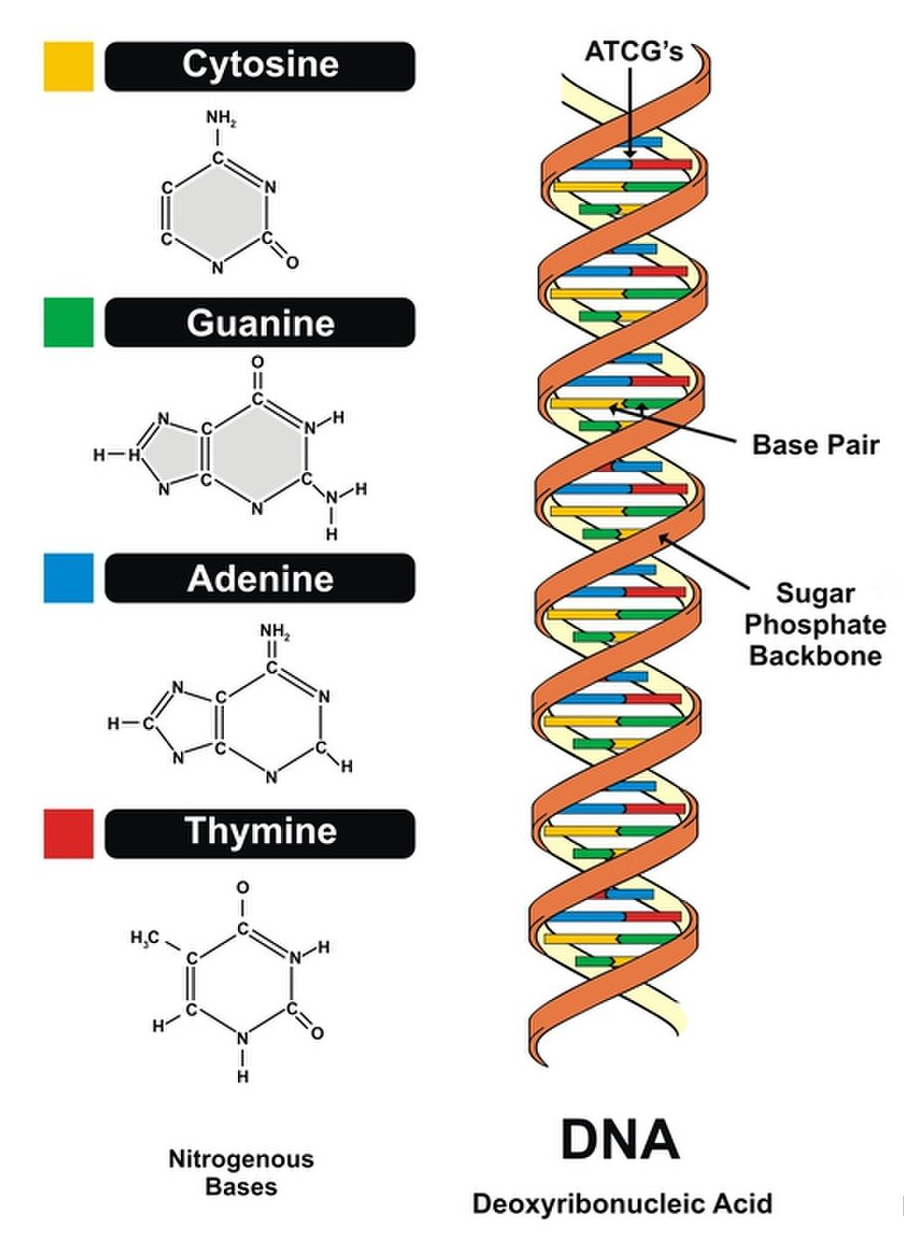
\includegraphics[width=200pt]{chapters/images/introduction/dna-structure.png}
    \caption{Structure of DNA}
    \label{fig:dnastructure}
%\end{figure}
\end{wrapfigure}

In humans, DNA is organised into 23 pairs of chromosomes, with a total length of over 3 billion base pairs. About 1\% of this DNA make up \emph{genes}; stretches of DNA which directly encode protein molecules. When these genes are expressed, the gene sequence is transcribed to a messenger molecule (\emph{mRNA}) which is subsequently translated into a protein molecule. The function of the remaining 99\% of the genome long remained a mystery, and was even referred to as \emph{junk DNA}. More recent studies have revealed that these stretches of non-coding DNA play an important role in the regulation of the expression of genes, stimulating or prohibiting the translation of genes to proteins and thereby influencing the functioning of the cell. For any two individuals, the vast majority of their DNA sequence will be identical, but small variations in the remaining locations of the genome are what make each of us unique. But it is also what can make us sick. Studying this natural variation in the genome sequence helps us unravel the mechanisms of life and disease.


\subsection{A Brief History of Genome Sequencing}
Friedrich Miescher was the first to isolate DNA molecules (which he termed \emph{nuclein}) in 1869. However, the molecule remained relatively understudied until Rosalind Franklin used X-ray crystallography to inspect the molecule's structure \cite{elkin2003rosalind}. Watson and Crick used this data (without credit) to postulate their double-helix model of DNA in 1953 \cite{watson1953molecular}. This model illustrated that DNA molecules could be replicated, and solidified the idea that DNA, and not proteins, was the primary carrier of hereditary information. Simultaneously, Frederick Sanger had developed techniques to sequence proteins, and later RNA and DNA molecules. This was the start of the era first generation sequencing. These early techniques enabled highly targeted sequencing of small stretches of DNA. The first full gene was sequenced in 1972 \cite{TODO}, followed by the first full genome in 1976. This was the bacteriophage Phi X 174 with a total length of 5386 nucleotides \cite{}.


In 1990, the Human Genome Project \cite{olson1993human} set out to sequence the entire 3.2-billion-basepair-long human genome, an effort culminating in 2003 with the publication of the first human \textit{reference genome} \cite{international2004finishing}. Not only did this provide invaluable insights into human genetics, but it also paved the way for the next era in genetic research; something which would completely transform the field of genetic research. Over the next several years, next-generation massively parallel sequencers were developed by companies like Roche454 and Illumina, dramatically cutting the cost and time required to sequence a human genome, and for the first time demonstrated its potential utility in clinical and diagnostic settings. Through sustained technological advancements over the following years, these costs continued to decrease at exponential rates - outstripping even the pace predicted by Moore's law (\hyperref[fig:seqcost]{Fig. \ref{fig:seqcost}}) - and the long dreamed-about \textit{\$1,000 dollar genome} \cite{thousanddollargenome} \cite{sequencingcostsNHGRI} has now become a reality.

\begin{figure}[h!]
    \centering
    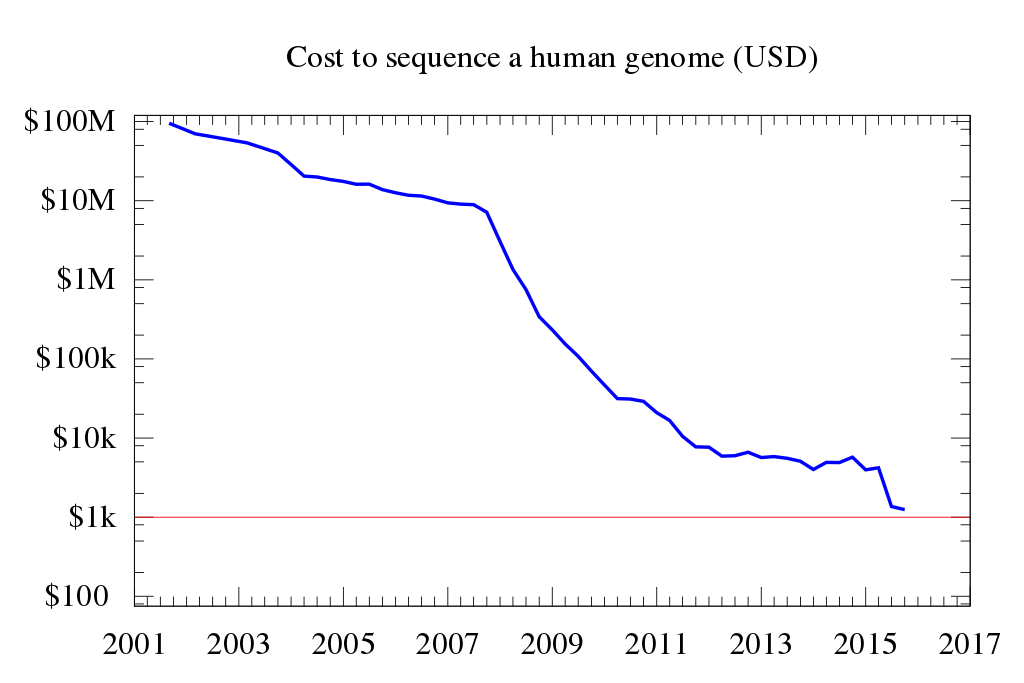
\includegraphics[width=300pt]{chapters/images/Historic_cost_of_sequencing_a_human_genome.png}
    \caption{The cost of sequencing a human-sized genome over time. Data from the NHGRI Genome Sequencing Program (GSP) }
    \label{fig:seqcost}
\end{figure}

Shortly after the publication of the human genome, high-throughput techniques emerged to also sequence the transcriptome (RNA-Seq), allowing for the identification and quantification of gene transcripts, and providing information about post-transcriptional mutations and other complexities such as alternative splicing \cite{wang2009rna}. Similarly, the study of epigenetics is revealing that non-coding DNA, far from the once-termed \textit{"junk DNA"}, is part of an intricate and complex regulatory system controlling the expression of genes \cite{zuckerkandl2007combinatorial}.

Now we are now moving into the era of third-generation sequencing, where single-cell \cite{gawad2016single}, long-read \cite{koren2015one}, and often real-time sequencing \cite{flusberg2010direct} are allowing for ever more accurate determination of nucleotide sequence, providing increased resolution even in highly diverse and complex samples such as tumours or metagenomic samples. All these technological advances have led to a deluge of data that must be managed and analysed, typically by bioinformaticians.


\section{The Bioinformatics Challenge}

With huge amounts of data now being generated at relatively low cost \cite{chen2014big}, and compute resources being available even on moderate budgets, the challenge in genomic research has shifted from the sequencing technologies to the analysis and interpretation of these big and highly complex datasets, and the development of the software required to do so, in order to gain new understanding of the underlying biological systems. This poses a significant challenge, both technologically and scientifically.

\subsection{Ever-changing landscape}
Sequencing technologies are evolving at a staggering pace, and with them, so must the software tools capable of analysing the data. Therefore, new tools are developed continually and existing tools must be updated regularly to remain relevant. As a consequence, there typically simply is not enough time for community standards and consensus analysis pipelines to emerge organically before the advent of new technologies make them obsolete. Because of this, there usually are a multitude of tools available for any given task, each with their own set of advantages and disadvantages, and the challenge is to find the right tool for the particular situation, and knowing when to use existing tools and when the development of novel tools is in order.

\subsection{Standardisation}
Such a lack of clear standards does not only apply to software tools, but also to file formats, and this poses a major hurdle in data analysis. While some clear data format standards exist [fastq, VCF], there are many cases that lack such a standard, hindering the interoperability of different tools. And even the more established file formats such as fastq and VCF allow for a variety of flavours, e.g. different fastq quality encoding schemes, which are not indicated inside the file format specification itself, but may influence downstream results. Thus, when creating analysis pipelines from existing tools, many file transformation steps are typically required as a kind of \textit{glue} between steps.

\subsection{Data Storage}
 \begin{comment} https://qumulo.com/blog/genomic-sequencing-qf2-storage/ \end{comment}
Sequencing data is being generate at a rate of X petabytes per year (TODO: find citation), and all this data must be stored somewhere. But there is more to data storage than buying a hard disk and copying data. The data must be backed up to prevent data loss, it must be made available for use in an efficient way (I/O matters), data must be organised and tracked in a usable manner, and any solution must be able to scale to the exponential trend of growth both in size and number of files generated. Furthermore, data storage must comply with privacy and security requirements, especially important in the case of human genetic data.


\subsection{The Specialist Bioinformatician}
All of these challenges have resulted in bioinformatics becoming a highly specialized field, which in itself poses a new challenge given the observation that the domain knowledge (biology) and the informatics know-how more and more often do not reside in a single individual, and the interpretation of the data cannot always be done by the person performing the data analysis and vice versa. Instead, close communication between the two fields is required, and the domain experts should be empowered to perform their own data analyses as much as possible.

\verb+informatician needs to shine a light in the black box that is the wetlab, domain expert needs to become comfortable with the informatics, since this has become an integral part of any analysis+


% some (partial) solutions to the above challenges, spoilers: open software, open science, open everything
\section{Bioinformatics Best Practices}
Since bioinformaticians are primarily academics -who are typically being judged on their publications, not their code-, the quality of bioinformatics tools is highly variable and tool authors often struggle to find the time and resources to maintain their code. The open-source community is instrumental in this respect, allowing the most popular and useful tools to be taken up by the community which can collectively maintain and update the bioinformatics software packages. Adhering to a set of best-practices guidelines can greatly reduce this maintenance burden, and increase the chance of tools being taken up by the community.

Many journals require authors to submit datasets to public repositories in order to allow other scientists to reproduce their findings. With bioinformatics now such a fundamental part of any publication, a clear description of the analysis pipeline is also required for true reproducibility, but the majority of scientific publication do not contain all the information required to reproduce the in-silico experiment [cite]. Making analysis software open-source and adhering to a set of bioinformatics best-practices can improve the reproducibility of bioinformatics analysis pipelines.

Such bioinformatics best-practices include:

\begin{enumerate}
    \itemsep-0.5em
    \item Accessibility of tools and data %(usability) of tools (documentation, open source, github etc, galaxy, galaxy, dependency management, docker)
    \item Reproducibility %(conda, docker, galaxy, version control, code notebooks)
    \item Interoperability %(data formats, common frameworks, generic, allow for packaging)
    \item Maintainability of software %(testing, continuous integration, community buildingi, scalability)
    \item Visualization and reporting
    %\item Data management and sharing %(FAIR data, LIMS, PIDs)
\end{enumerate}


\subsubsection{Accessibility}
Most bioinformatics tools are commandline unix tools, and biologists are not typically trained in the use of such. Even for the experienced bioinformatician, running some of these tools can be a challenge due to lack of documentation or quality of the tool. Ideally, once a tool or pipeline has been validated, the analysis can be run by the domain expert, i.e. the research scientist responsible for the interpretation of the analysis results, without being reliant on the support of a bioinformatician at every step \cite{kumar2007bioinformatics}.

Creating user-friendly software is not a trivial task. Application linking (also referred to as wrapping), can ease this burden for the tool developer. In such an approach, existing user-friendly interfaces host third-party software packages -at miniumum effort to the developer of the hosted software- and thereby offer a layer of abstraction to the end-user that shields them from the implementation details of the tool and provides a uniform usage paradigm for all tools, regardless of their differences behind the scenes. Examples of such hosting frameworks in the context of bioinformatics are Galaxy \cite{giardine2005galaxy,goecks2010galaxy}, Taverna \cite{}, [more?].

Accessibility also includes high-quality documentation of the tool, both for developers and end-users, and ideally some form of training manual to educate users in the proper use of tool and warn about possible pitfalls and biases.

\subsubsection{Reproducibility}

A cornerstone of the scientific method is reproducibility of results. Experiments should be described in sufficient detail to allow for their reproduction and independent verification by fellow scientists. In reality however, this remains a big challenge, and many publications can not be reliably reproduced based on the information provided in publication []. In many cases this holds not only for the wetlab experiment, but also for the in-silico downstream data analysis. Reproducing bioinformatics analyses often becomes an exercise in \textit{"forensic bioinformatics"}; trying to piece together the exact procedure used through trial and error and educated guessing. In part this is caused by journals not having clear submission guidelines for bioinformatics pipeline description as they do for the physical samples. The latter are commonly required to be submitted to biobanks before submission, and the raw datasets generated from them to be stored in online repositories. No such requirements are generally imposed on the downstream analysis, or when they are these requirements are not strict enough to ensure true reproducibility. This is not without consequences; in some cases this has lead to clinical trials being started based on incorrect conclusions not revealed during peer review due to lack of reproducibility \cite{baggerly2009reproducible}.

% dependency management
But even if the full source code were made available, reproducibility of the entire dependency chain of all software and system libraries used remains problematic. Every package in this dependency tree has the potential to influence the final result. While reproducibility is a high priority in the scientific community, this isn't the same for software developers in general, and many packages will simply be removed when an update has been made available. This is where package managers such as Conda \cite{gruning2017bioconda} or GNU Guix \cite{courtes2013functional} offer significant improvement, by allowing specific versions of tools to be installed, and mandating that any changes made to a package must be submitted as a new version, and existing version remain available and unchanged indefinitely. This ensures that the stack of software obtained when installing a tool at a specific version will yield identical results today as it will a year from now.

% provenance
Once the correct set of software is obtained, the provenance of how the tools were applied to the data must also be logged. This includes the sequence and interplay of different tool executions, with the full parameter settings and input and reference data used at every step. Keeping a lab journal of the in-silico experiment is a good start, but too error-prone as a manual process. Projects such as Jupyter Notebooks \cite{kluyver2016jupyter} for Python, or Sweave \cite{leisch2002sweave} and KnitR \cite{xie2014knitr} for R, allow for the mixing of text and tools to create interactive journal articles if you will, where the calculations are embedded within the manuscript, and these calculations can be examined and rerun or adjusted with ease. A drawback of this of course comes when tools require a lot of resources or are not all written in the same language, as is typically the case for NGS analyses. Workflow platforms such as Galaxy \cite{} automatically keep track of provenance for the user and have the advantage of supporting a wide range of tools.


\begin{comment}
"forensic bioinformatics" -> have to figure out by trial and error what was done

https://bmcmedresmethodol.biomedcentral.com/articles/10.1186/s12874-017-0377-6
https://www.biostars.org/p/52561/
https://www.nature.com/naturejobs/science/articles/10.1038/nj7396-137a
https://www.nature.com/nm/journal/v13/n11/full/nm1107-1276b.html
\end{comment}

\subsection{Interoperability}

A plethora of bioinformatics tools are available, and most analyses require combining a number of tools together into an analysis pipeline, also referred to as a workflow. The different components in such a pipeline usually do not work seamlessly together without a bit of "glue"; custom scripts that convert the output of one tool so that it can be used as input for the next. This is necessary due to the frequent lack of clear data formats. For example for structural variations, no clear data format exists, and most tools output custom formats. Many of these custom formats contain the same information, it is often formatted differently. Any tools working on such datasets make assumptions about its format, so we must take care to adhere to these expectations. Even in cases where file formats are more standardized, variations in the exact implementations may still require careful consideration within a pipeline. Consider for example the fastq format; this is a relatively simple format, just 4 lines per sequence read, but the fourth line, the line containing quality score, is the source of some divergence in the format. A range of ASCII characters is used to encode numerical values indicating a PHRED-like quality score of the base call, but the range and start position of this character range comes in different flavours. Furthermore, because these ranges overlap, it is not always possible to deduce which convention was used unless some quality encoding are present in the file that only appear in one of the conventions. It is therefore important to know the convention used for any datasets entering your pipeline, and know when tools make assumptions about their input data. If necessary, a format conversion step can be employed to resolve any mismatches between the format expected by a tool and the format of the input dataset. Similar widespread variations in standard formats include chromosomal location (0-based or 1-based numbering, open or closed) and chromosome names (with or without a `chr` prefix). These issues are not hard to deal with, but can lead to inaccurate results if not carefully taken into account by the creator of the pipeline.

% packaging
On a more technical level, different tools may be written in different programming languages and/or compiled for different operating systems, and it can be a challenge to combine these into a single analysis. Luckily, tool developers can undertake steps to make their tools more interoperable. Package managers such as bioconda will compile software from its source for different operating systems. For bash scripts, many OS-dependent syntax variations can hinder interoperabililty, but by taking care to comply with POSIX standards, such concerns can be mitigated. Vitally, precise documentation of any assumptions made in the code is indespensible, and making source code open further facilitates this transparancy.


\begin{comment}
file format standards, common frameworks, good documentation, open-source,
allow for packaging (don't deliver code as VMs etc),
\end{comment}

\subsection{Maintainability}
In bioinformatics, the emphasis for scientific accomplishments is placed on scientific publications, not on software products. As a result, many tool developers struggle to find the time and resources to maintain their software beyond its release. Since scientific research depends increasingly on these pieces of software, decreasing the burden of tool maintainence is valuable and worthwhile pursuit. Furthermore, many tools are written by small research groups or single individuals who are simply unable to perform the necessary maintainence without support. By making tools open-source, the entire bioinformatics community is able to step up as co-developer, allowing them to discover bugs and contribute fixes or enhancements. Code sharing platforms like GitHub \cite{} and BitBucket \cite{} facilitate this community-driven approach to software maintainance.

Using code versioning such frameworks such as git \cite{} or mercurial \cite{} ensures precise tracking of changes and ability to revert to any previous state at minimal effort, and facilitates merging of that Incorporating tests at every phase of development can further decrease the maintenance effort. Unit tests ensure that small code modules show expected behaviour at all times. Functional tests ensure that these different units of code always yield the desired result when working in conjunction. Code quality checks can help streamline the code itself and increase readability, benefiting future development. Continuous integration is the paradigm whereby changes to the mainline code are incorporated incrementally and continually, and thoroughly reviewed and tested at every stage.

%versioning continuous integration, functional testing, code review, dependency resolution (conda)

\subsection{Visualisation and Reporting}

As scientists become increasingly reliant on large and complex computational analyses in their research \cite{chen2014big}, the final analysis result datasets become similarly complex and have  often grown beyond the realm of what can be manually viewed and interpreted, both in terms of the number of files and their sizes, as in terms of complexity. Analysis results therefore require summation and visualisation and must be presented to the domain expert in a comprehensible and accesible manner. Such a report should also contain detailed descriptions of the methods used and assumptions made and citations to any third-party tools employed, as an understanding of these factor can assist in interpretation \cite{kumar2007bioinformatics}.

For genomics data, visualisation tools such as Circos \cite{circos} [list more examples] enable the integration of various output datasets, often in the order of millions of lines each, to be summarized in a single image. While some resolution may be lost in such visualisations, they do enable the easy identification of areas of interest and guide the interpretation by pointing the domain experts in the direction of further inspection.


\section{The Galaxy Project}
The Galaxy project \cite{afgan2016galaxy} facilitates many of the best-practice bioinformatics guidelines outlined in the previous section. Galaxy provides a graphical web-based interface to commandline bioinformatics tools, bringing the data analysis to the domain experts equipped to perform the interpretation of the results. With its heavy focus on accessibility and reproducibility, Galaxy is an important component in creating high-quality bioinformatics pipelines. Galaxy keeps track of the full analysis provenance, manages tool dependencies with bioconda \cite{}, has built-in visualisations, and is accesible by end users with nothing more than a browser. For developers, Galaxy provides a convenient framework to package tools to make these available for researches throughout the global community. The Galaxy toolshed

\section{Training}
With -omics research becoming increasingly computational in nature, and many research groups not having access to a dedicated bioinformatician, there is a great need for high-quality bioinformatics training to ensure that the domain experts who interpret the results of data analyses are optimally equipped to do so. Surveys confirm this need for bioinformatic training; the majority of researchers (>95\%) work with or plan to work with large datasets, but most (>65\%) possess only minimal bioinformatics skills and are not comfortable with statistical analyses \cite{larcombe2017elixir}, \cite{williams2017vision}. Demand for training currently greatly exceeds the supply \cite{attwood2017global}. In a recent survey \cite{survey2013embl} over 60\% of biologists expressed a need for more training while only 5\% called for more computing power. Thus one can assume that the true bottleneck of the current data deluge is not storage or processing power, but the knowledge and skills to utilize existing resources.

With its focus on accessibility and user-friendliness, the Galaxy platform is also an ideal environment for teaching. Trainees are shielded from the minutia of the implementation details of the underlying tools, and need nothing more than a browser to execute the tutorials. Because Galaxy can host any commandline tools and the tools available in the tool shed cover a wide range of topics, creation and maintainence of a set of training materials must be a a community effort, with content being created by a large number of people with expertise in the various topics.

[TODO: slightly plagiarized from my own paper, rephrase?]

\newpage
\thispagestyle{empty}
\begin{center}
\vspace{2cm}
\begin{minipage}{6in}
\tikz[remember picture,overlay]
\node[opacity=0.8,inner sep=0pt] at (current page.center){
    %
\includegraphics[width=\paperwidth,height=\paperheight]{chapters/images/background-texture-blue.jpg} %higherquality image but too big for overleaf
    
\includegraphics[width=\paperwidth,height=\paperheight]{chapters/images/background-texture-blue-reduced.jpg}
};
\sc
\begin{center}

\color{white}{
\Large Prostate Cancer \normalsize
\vspace{2cm}


I like puzzles. Any type of puzzle. I always have. If I see a puzzle or a problem I have to solve it. I think that is what makes cancer such a fascinating topic for me.

\vspace*{0.5cm}

Imagine you are given a jigsaw puzzle. Now instead of a few hundred pieces, there are several billion pieces. The picture on the box is not a picture of the puzzle inside the box,
it is just a somewhat similar image. Oh, and did I mention there are a whole bunch of pieces missing? and that many pieces are duplicated? Some pieces don't even belong in our box,
but come from a completely different puzzle. On top of that your little sister has spilled paint over some of the pieces so those can't be trusted to contribute to the image. And instead of one
single puzzle, the box contains several, they are all variations of the image on the box, but you have no idea how many different puzzles the box contains. Sound challenging? This is the problem we are solving whenever we sequence a cancer genome.

\vspace*{0.5cm}
\textbf{[Metaphor key]} \\
\textit{puzzle pieces} = sequence reads \\
\textit{picture on box} = reference genome \\
\textit{missing pieces} = hard-to-sequence areas \\
\textit{other puzzles} = contamination \\
\textit{painted pieces} = sequencing errors \\
\textit{multiple puzzles in box} = clonality
}

\end{center}
\end{minipage}
\end{center}



\newpage
\section{Use case 1: Prostate Cancer}

\epigraph{3in}{The time has come in America when the same kind of concentrated effort that split the atom and took man to the moon should be turned toward conquering this dread disease.}{President Richard Nixon}

On December 23, 1971, President Richard Nixon, buoyed by recent technical feats such as the moon landing, signed into law the National Cancer Act, thereby declaring a war on cancer. Today, more than 45 years later, that war is still being waged in full force. While great advancements have been made towards this goal, some of the initial optimism has been quelled by discoveries of the great complexity and heterogeneity underlying cancer.


\subsection{The Hallmarks of Cancer}

Tumor cells evolve from normal cells through the acquisition and accumulation of mutations. The human body has mechanisms in place to repair or dispose of damaged cells and to prevent runaway cell division, so in order for a tumour cell to survive and thrive it needs to acquire changes that provide it with advantages for proliferation and evasion of the cell's defense mechanisms. Evidence suggests this transformation from healthy cells into malignant cells follows a strikingly similar path across all different tumour types \cite{}. A cell's acquired abilities that drive tumour progression are know as the \emph{hallmarks of cancer} and consist of the following six characteristics:

\begin{itemize}
    \itemsep-0.5em
    \item self-sufficiency in growth signals
    \item insensitivity to anti-growth signals
    \item evasion of programmed cell death
    \item limitless replicative potential
    \item sustained angiogenesis
    \item tissue invasion and metastasis
\end{itemize}

Each of these steps overcomes one of the body's anti-cancer defense mechanisms. This evolution into malignancy is an almost darwinian process where the mutations acquired are random, but those cells that have gained mutations which are advantageous for survival will be able to replicate and thrive and accumulate further mutations. Distinguishing the mutations that impart a strategic advantage and thereby \emph{drive} a tumour's progression, from the often huge number of less harmful \emph{passenger} mutations accumulated over the lifetime of a cancer cell is no easy task. The optimal course of treatment for a patient often depends on the mutations present and how the cell functions are subsequently impacted by those mutations. However, many different mutations may lead to the same disruptions of key pathways, therefore we must evaluate mutations not just at the DNA level but in the broader context of their functional impact on the cell's internal processes.



\subsection{Cancer's Complexities}

Determining the exact genetic sequence of healthy individuals is already quite a challenging endeavor; trying to extend this to cancer genomes takes this challenge to the extreme. There are several complexities present in cancer geneomes that make accurate determination of the genetic changes and their downstream impacts a difficult task:

\begin{enumerate}
    \itemsep-0.5em
    \item Small variants
    \item Structural variations
    \item Clonality
    \item Temporal Evolution
    \item others? Epigenetics? transcriptome level complexities?
\end{enumerate}

In the following sections we will discuss each of these complexities and explore the biological and informatics challenges posed by them.

\subsubsection{The Bio}
\paragraph{Small variants} comprise the simplest class of mutations; those consisting of alterations of just a handful of bases, for instance the \emph{substitution}, \emph{deletion} or \emph{insertion} of one or more nucleotides.

The impact of such mutations depends on where in the genome they occur. Single nucleotide variants (SNVs) in exonic regions can range from having no effect on the resulting protein (silent) to changing an amino acid in the protein to a different amino acid (missense mutations), to changing a codon into a stop codon (nonsense mutation) which nearly always results in a nonfunctional protein. If this happens in a protein that is vital to the functioning of the cell this can have disastrous consequences <some examples of SNVs causing serious problems/phenotypes> <conserved regions, cell's mechanisms for preventing such fatal flaws>

These simple variations were the first to be extensively studied and found to contribute ..

While variants within the coding sequence are most likely to have an impact on cell health, small variants \emph{outside} the coding sequence can also have drastic impact on health, for example 70\% of melanomas exhibit a point mutation in one of two positions in the promoter region of TERT (Horn et al. 2013; Huang et al. 2013).

\paragraph{Structural variations} are larger-scale mutations, involving rearrangement of segments of DNA of more than roughly 50 bp. These often do not involve the coding sequences directly, and can therefore only observed through whole-genome sequencing. Such structural variations can lead to changes in regulation,

<fusion genes>


\paragraph{Clonality}


\paragraph{Temporal Evolution}
\paragraph{Epigenetics}

\subsubsection{The Informatics}

We know that changes in sequence and structure of DNA contributes to cancer development. But how do we describe these properties? Any two healthy individuals differ greatly in their DNA sequence; it's what makes us us. How to denote these differences is a non-trivial problem, as is determining which of these differences are just part of the natural variation between individuals and which are ones detrimental to our health and functioning.

If you were asked to describe the differences between two Shakespeare plays, how would you go about it? They are made up of the same alphabet, and share many of the same words and even whole sentences, but to list the differences between them can be done in many ways. You could number the words in both books and take note of the ones that are different in each position, but then if you were to take two identical sentences and prefix one with a single extra word, all positions would end up being flagged as different while clearly these sentences are nearly identical. And ..

<note: ditch the book analogy? example shakespearean sentence to illustrate? >

poor concordance between variant callers: https://genomemedicine.biomedcentral.com/articles/10.1186/gm432


Currently variations in DNA are described relative to a \emph{reference genome}; a sequence intended to represent the \emph{average} human genome, which was constructed by taking the most frequently observed nucleotide at any given  position in the genome
<discuss some drawbacks/things to realize: based on relatively small set of samples, not optimally diverse set of individuals>

As we have seen, the choice of software can impact downstream analysis, and variant calling is no exception. Different aligners employ different mapping strategies, which leads to different variant calls for the same observed sequence depending on the choice of algorithm, complicating variant comparisons between studies \cite{zook2014integrating}. While there do exist tools to canonicalise some of these differing representations \cite{vcflib}, complex variants remain that do not have a single obvious standard form (Figure \ref{fig:variant-multiple-representations}).
But even for the simpler cases, there is not always a clear consensus on how to standardise representation. Consider for instance the case where an adenine nucleotide has been inserted, transforming the sequence \verb+TAAG+ to \verb+TAAAG+. Do we describe the insertion to have happened at position 1 (after the \verb+T+), position 2 (between the two \verb+A+s), or at position 3 (before the \verb+G+)? While this particular case is easily solved by agreeing on a convention of either left-aligning or right-aligning these variants, such community agreement does not currently exist, with most next-generation analysis tools opting for left-alignment, while certain variant databases such as HGVS [TODO cite] still recommend (but do not enforce) alignment to the position nearest the 3\` end of the gene \cite{hgvs-position}, which translates to right-alignment in genomic coordinates for reverse strand genes. Furthermore, once variants have been submitted to online databases, information about surrounding variants observed in the same sample is often not kept, making it impossible to resolve equivalency of variant representations going forward.

\begin{figure}[h!]
    \centering
    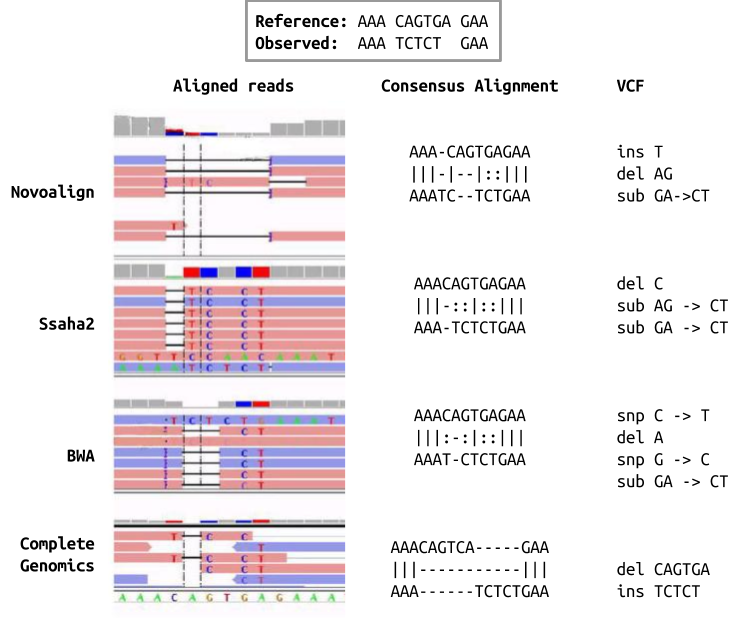
\includegraphics[width=400pt]{chapters/images/variant-representation-all.png}
    \begin{comment}
        image in google drive https://docs.google.com/drawings/d/1WWmzW6uWtJ7HZ5WVgtg_oAMA_3E_569M4Ikjz4Ecjic/edit
    \end{comment}
    \caption{Complex variants can be represented in multiple ways. Four different aligners (Novoalign, Ssaha2, BWA, Complete Genomics) treat the same variant in vastly different ways, which leads to such differing sets of variant descriptions in the VCF files that it is no longer apparent that these variants in fact describe the same observed sequence.}
    \label{fig:variant-multiple-representations}
\end{figure}


<not to mention sequencing errors, at rate of abt x/100, sequencing depth helps but tradeoff with cost>

sources of mismatch with reference genome \\
- real mutation \\
- wrong base call \\
- wrong mapping/variant call \\


<repetitive regions>

The result of all of this is that different variant calling tools will produce different sets of variants given the exact same input dataset and reference genome, and it is hard to know who does a better job, if their respective papers are to be believed each one of them far outstrips all the others. But as with everything in life, the truth lies somewhere in the middle. Each of the variant callers has its strengths and weaknesses, some may very accurate in calling one type of variant but have  more difficulty with others. Some are very accurate in healthy genomes but less so in highly mutated genomes or vice versa. One possible solution is to run a set of variant callers

\paragraph{Structural variations}
<very very poor overlap between different methods>

<hard to resolve exact location of junctions>

<chainfinder>
\paragraph{Clonality}
\paragraph{Temporal Evolution}
\paragraph{Epigenetics}



\newpage
\thispagestyle{empty}
\begin{center}
\vspace{2cm}
\begin{minipage}{5in}
\tikz[remember picture,overlay]
\node[opacity=0.8,inner sep=0pt] at (current page.center){
    
\includegraphics[width=\paperwidth,height=\paperheight]{chapters/images/background-texture-blue-reduced.jpg}
};
\sc
\begin{center}

\color{white}{
\Large The Human Microbiome \normalsize
\vspace{2cm}

When Dutch inventor and scientist Antonie van Leeuwenhoek first turned his microscope to a drop of rain water and discovered within a wealth of microscopic life which he termed \textit{animalcules}, a whole new world of knowledge opened up. Soon after, it was discovered that while these organisms might be microscopic in size, their impact on human lives was enormous, causing food to spoil and disease to spread. Through the study of these micro-organisms, scientists were able to develop methods for enhanced food preservation and eventually also new treatments and vaccines for a whole range of illnesses.

Cost of sequencing has now dropped enough that it has become feasible to sequence not only a patient's own DNA, but also the DNA of their microbiome to make a diagnosis or to determine the best treatment option.




\vspace*{2cm}
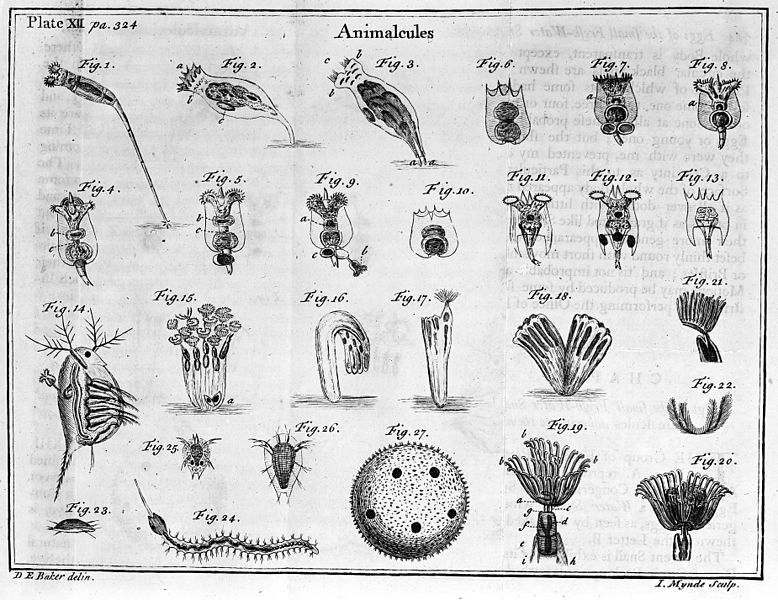
\includegraphics[scale=2]{chapters/images/mycrobiota/animalcules2.png}

}

\end{center}
\end{minipage}
\end{center}

\newpage


\section{Use case 2: Microbiota}

\begin{comment}

overview of reading materials about the human microbiome

http://www.richardsprague.com/note/2017/10/16/best-academic-papers-about-the-microbiome/

informal history of microbiology: https://www.bioexplorer.net/history_of_biology/microbiology/
\end{comment}

\subsection{The Bio}
first complete bacterial genomes published in 1995  \cite{land2015insights}

16S rRNA

whole genome shotgun

\subsection{The Informatics}


\begin{comment}
history of microbiolgy: https://courses.lumenlearning.com/boundless-microbiology/chapter/introduction-to-microbiology/

<WGS reveals changes outside coding regions, such as one affecting regulation of genes are of importance, and can reveal large scale changes (SVs), fusion genes>

<epigenetics>

<potential of developing treatments from all this knowledge>

sources:
- Hallmarks of cancer: the next generation [@hanahan2011hallmarks]
- Chromosome aberrations in solid tumors [@albertson2003chromosome]

~~~
low-resolution methods:
- fluorescent in sit hybridisation FISH [Pinkel et al 1988, Thompon and Gray, 1993]
- chromosome painting [Jauch et al, 1992]
- spectral karyotyping [Schrock et al 1996]
- comparative genome hybridisation CGH [Kallioneimi 1992]

- arrays

high-throughput:
 - LOH [@hampton1996simultaneous]
 - GWAS

 - 2003 still infeasible to sequence entire tumor genome, so
   ESP (end sequencing profiling) used [Volik et al 2003]
       (- BAC library from tumor, sequence ends, map to reference)
    → reconstruction from ESP data [Rapael et al 2003]

now: WGS
- NGS: DNA short reads
- NGS: RNA Seq
- NGS: Paired end mapping [@korbel2007paired]
- limitations of current methods
~~~

advanced in cancer research specifically from next generation methods: [@meyerson2010advances]

\end{comment}







\begin{comment}

types of SVs: standard, complex, chromothripsis [@stephens2011massive]

- well-known examples
    - TMPRSS ERG
    - ABL gene on chr9, chronic myeloid leukema, translocation between chr9 and 22,
       changes regulation, promotor becomes promotor of BCR gene on chr22
      [Heisterkamp et al 1983]

#### usefulness in biomarker and treatment development

- Gleevec, targeting BCR-ABL fusion gene [@druker2001efficacy]
- Herceptin, targeting ERBB2 amplification [@kauraniemi2004effects]


#### SV Tools and databases

~~~
- catalogued in Mitleman database [Mitelman 2003]
- COSMIC
- ..
~~~

## Clonality

## Temporal evolution

## etc..
~~~
<Informatics/analysis methods>
 - History of methodologies (gwas, ..)
 - NGS: Huge datasets, excel and manual analyses no longer suffice
 - Cancer: Germline correction, drivers vs passengers

<Limitations of current methods>
 - imperfect data
 - disagreements and biases per lab/informatics technique

<Challenges in tumour genome reconstruction>
→ explain in biology section, here describe why that complicates things

 - Normal Contamination
 - Clonality detection
 - Event Chains detection
 - Temporal evolution detection


\end{comment}

\section{Scope of this Thesis}
Bioinformatics is a vital part of many fields of research. While these may differ greatly in the biology involved, many of the bioinformatics concepts are shared among them. In \hyperref[chapter:general]{Chapter \ref{chapter:general}} we discuss several such widely-applicatble bioinformatics projects. Galaxy for reproducible analysis workflows, iReport for results reporting withing Galaxy. (Circos? myFAIR?)



\bibliographystyle{ieeetr}
\bibliography{references}
